\documentclass[10pt,twoside,twocolumn]{article}
\usepackage[bg-print]{dnd} % Options: bg-a4, bg-letter, bg-full, bg-print.
\usepackage[utf8]{inputenc}
\usepackage[super]{nth}
\usepackage{calligra}
\usepackage{makeidx}
\usepackage{multind}
\usepackage{fourier}
\usepackage{graphicx}
\makeindex{locations}
\makeindex{characters}
\makeindex{monsters}

% Start document
\begin{document}
\fontfamily{ppl}\selectfont % Set text font

\section{Session 1,  May 7\\\textit{Where's the Baby?}}
\subsection{Daggerford}
We find ourselves in \textsc{Daggerford}\index{locations}{Daggerford}, at the \textsc{Pickled Inn}\index{locations}{Pickled Inn}. Locals have been
asking for mercenaries to help with a ``werewolf problem.''

\begin{commentbox}{The Pickled Inn}
  \textit{Ragnar}\index{characters}{Ragnar} has inherited the inn from his \nth{2} cousin. He is now bragging
  about his newfound fortune.
\end{commentbox}

\textit{Orva}\index{characters}{Orva} tasks us with finding the source of the werewolf raids. Every
night, a fog rolls in from the \textsc{Misty Forest}\index{locations}{Misty Forest}, as werewolves\index{monsters}{werewolf} emerge,
kill adults, steal children (8 and under) and return to the
forest. There's a \textbf{reward of 500 gp for finding their lair, and 20
gp/ear}. We get some items, and head south approx. 100 miles to the
fortified roadside inn, the Blue Fox.

\subsection{The Blue Fox}
Four days of travel south on the tradeway brings us to the \textsc{Blue Fox}\index{locations}{Blue Fox},
where we learn more about werewolves.

\begin{commentbox}{The Blue Fox}
  The innkeeper is a half-elf retired cartographer named \textit{Olga}\index{characters}{Olga}. Has an
  assistant half-orc named \textit{Todd}\index{characters}{Todd|seealso{Olga}}. Olga is Orva's cousin.
\end{commentbox}

\begin{paperbox}{Werewolves}
  Werewolves have three forms: humanoid, hybrid and wolf. Their
  ability to change is unrelated to the moon. They often disguise
  themselves as hunters or trappers.
\end{paperbox}

\begin{paperbox}{The Panther}
  There are whispers about ``The Panther''\index{characters}{Panther} robbing people on the
  tradeway. He or she likes to dress in purple and black silk.
\end{paperbox}

Slash finds an awesome carrion crawler skin drum, and Salvatore stocks
up on rations. We spend a quiet night, then continue into the
woods\ldots

\subsection{The Misty Forest}
We find some werewolf tracks, and follow them. 2 hours in, the tracks
have disappeared. A heavy fog descends, making it almost impossible to
see, and making us feel tired. We escape the fog. Quarion Speaks with
Animals, which have a forboding message:

\begin{quotebox}
  Woe to you that enters his domain.
\end{quotebox}

\begin{monsterbox}{Zombies}
  At the end of the path, we see a young boy and girl, and 2
  zombies. We successfully chase off the zombies.
\end{monsterbox}
We learn that the children are \emph{Thorn} and \emph{Rose}.\index{characters}{Durst family} Their parents
(\emph{Gustav} and \emph{Elizabeth}) trapped another zombie in the basement of
their home. \textbf{Baby brother \emph{Walter} is trapped on the \nth{3} floor of the house.}

Far off in the distance, we can see a castle, and are told that \emph{Baron
Strahd}\index{characters}{Strahd, Baron} lives there.

\subsection{Barovia}
\index{locations}{Barovia} Rose and Thorn lead us to their
house. Salvatore stays outside with the children. We go to the \nth{3}
floor of the house, where we find that the baby is just a bundle of
rags. Painting implies Elizabeth is not Walter's mother.

\begin{monsterbox}{Maid}
  In the nursery, we fight a woman who doesn't look quite
  right. Close inspection reveals that she has died a violent death.\index{monsters}{Spectre}
\end{monsterbox}

We finish exploring the \nth{3} floor, and proceed to the \nth{4} floor. \textbf{We
find the children's room with skeletons of the children}. We proceed through
a secret passage to the basement. The ghosts of Thorn and Rose appear
and possess Quarion and Slash.

\subsubsection{Basement}
We go left, then left again. We see human footprints and hear a
chant. We enter the ritual room.

\begin{monsterbox}{Shambling Mound}
  We fight a giant refuse pile named Llorgath.\index{monsters}{Shambling Mound}
\end{monsterbox}

After the battle, \emph{13 hooded, faceless figures} appear and start chanting:\index{characters}{Cultists}
\begin{quotebox}
  One must die, one must die\ldots
\end{quotebox}
\clearpage
\section{Session 2, May 13\\\textit{One raspberry, ple --- z\textsuperscript{z\textsuperscript{z}}}}
\subsection{Barovia}
\index{locations}{Barovia}

We clear the basement, return the children and maid bones, activate a
statue to Osybus, and find miscellaneous items, including the deeds to
the mill and the house.

\begin{monsterbox}{Ghouls}
  We defeat 4 ghouls, a grick and Gustav \& Elizabeth.
\end{monsterbox}

We discover that the Dursts were part of the \emph{Priests of Osybus}, and were sacrificing people to show their devotion. Their tomes and artifacts were bogus.

\begin{quotebox}
  {\calligra
  My most pathetic servant,
  
  I am not a messiah sent to you by the Dark Powers of this land. I
  have not come to lead you on a path to immortality. However many
  souls you have bled on your hidden altar, however many visitors you
  have tortured in your dungeon, know that you are not the ones who
  brought me to this beautiful land. You are but worms writhing in my
  earth.

  You say that you are cursed, your fortunes spent. You abandoned love
  for madness, took solace in the bosom of another woman, and sired a
  stillborn son. Cursed by darkness? Of that I have no doubt. Save you
  from your wretchedness? I think not. I much prefer you as you are.

  Your dread lord and master,

  Strahd von Zarovich}
\end{quotebox}

In town, \emph{Morgantha}\index{characters}{Morgantha} is trading dream
pastries for children. Barry eats a pastry and is
out. We learn that the pastries are created by a fey creature, with abjuration.
\\\\
\centerline{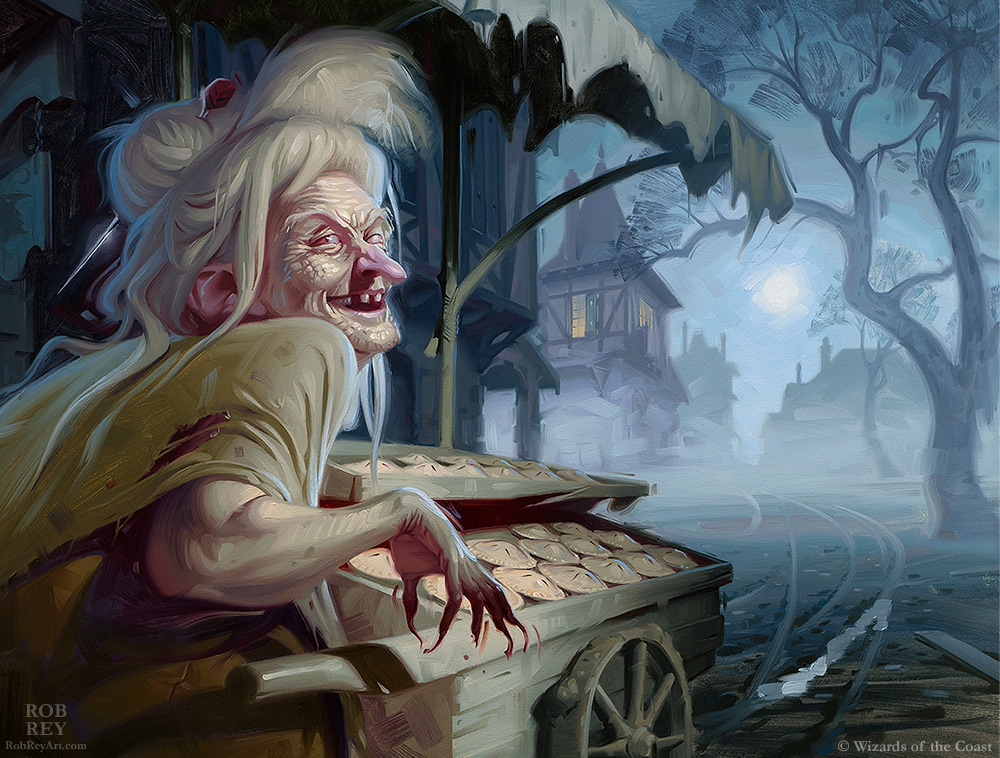
\includegraphics[width=0.85\linewidth]{morgantha}}

\subsubsection{Blood on the Vine Tavern}
\index{locations}{Blood on the Vine Tavern}
\textit{Ismark}\index{characters}{Ismark} is the mayor's son. The
mayor has an adopted daugher,
\textit{Irina}\index{characters}{Irina}. She's the focus of attention
from Strahd. \textbf{Ismark wants to move Irina to }\emph{Vallaki}\index{locations}{Vallaki}. Strange creatures
have haunted her house, and moving her would move her out of the
shadow of the castle.

Ismark promises us his family seal for helping.

\emph{Madam Eva}\index{characters}{Madam Eva} is a fortune-teller west of Barovia.

\begin{paperbox}{Baron von Strahd}
Morgantha tells us that Strahd has mastery over the land and the
weather, that he has undead enemies in Barovia. She talks of the
Fallen Knights of the Order of Silver Dragon\index{characters}{Fallen Knights of the Order of Silver Dragon}. Strahd has a very carefully
guarded secret: there is forbidden lore hidden in the mountains,
hidden in a temple.
\end{paperbox}

\begin{paperbox}{Werewolves}
  Ismark tells us that werewolves are under the control of Strahd.\index{characters}{Strahd, Baron} There's a pair of brothers that live in Valachi that hunt werewolves.
\end{paperbox}

\begin{paperbox}{Vistani}
  There's a camp to the west, and another one in the outskirts of
  Vallaki. Vistani are spies for Strahd, many are fortune tellers. They
  own the Blood on the Vine Tavern.
\end{paperbox}
\clearpage
\section{Session 3, June 3\\\textit{Security Questions}}
\begin{paperbox}{Baron von Strahd}
  $\hdots$ is a vampire! And can summon wolves and vermin. He can transform into a cloud of mist.
\end{paperbox}
Visiting the mayor's house, we find that he's been dead for 5 days. Danovich\index{characters}{Danovich (priest)} is the priest at the local church. We learn that there are two gods here: Morning Lord and Mother Night. His son stormed castle Ravenloft after being lured by a wizard in black robes. He thinks the wizard is dead, and the son has returned as a vampire spawn. After a funeral for the mayor, we head to the Vistani camp.
\subsection{Vistani Camp}
On the way, we scare off some nice trappers who were certainly not werewolves. Speak with a raven, who tells us to go to the \emph{Blue Water Inn}\index{locations}{Blue Water Inn} in Vallaki\index{locations}{Vallaki}. We meet Madam Eva\index{characters}{Madam Eva}, who reveals tarot cards telling us that:
\begin{paperbox}{Tarot Cards}
  \begin{itemize}
  \item Treasure lies within a mill.
  \item What you seek lies at the crossroads of life and death.
  \item The Sword of Sunlight is a weapon of vengeance. Look for it at an evil tree which grows atop a hill of graves where the dead ones sleep. Ravens can help us find it.
  \item To find an ally, look for a man of music with 2 heads who lives in a place of hunger and sorrow.
  \item Our enemy is a creature of darkness. Card of the temptress will lead us to him. A secret place, a vault of temptation hidden behind a woman of beauty. Evil lays atop his tower of treasure.
  \end{itemize}
\end{paperbox}
\begin{paperbox}{Wizard}
  1 year ago, the Wizard thought he could rally the people of Barovia against Strahd. The vampire appeared, the peasants fled. The vampire and wizard cast spells at each other. The wizard survived. ``Mad Mage of Mount Baritok''
\end{paperbox}
We also find out that a skeletal rider perished trying to escape the fog. We see a large black carriage, drawn by 2 black horses, which does psychic damage when attacked. Perhaps Strahd's.
\subsection{Blue Water Inn}
\begin{commentbox}{Blue Water Inn}
  Innkeeper Irvin Martikov\index{characters}{Irvin Martikov}. Really likes ravens.
\end{commentbox}
The burgermeister of Vallaki is Baron Vargas Vallokovich\index{characters}{Vargas Vallokovich}. Lots of festivals might keep Strahd at bay.

Watcher family (Lady Watcher and her two sons, Karl and Nikolai\index{characters}{Watcher family}) have old ties to Strahd and are enemies with the burgermeister.

Finally, we learn of Izak Strazni\index{characters}{Izak Strazni}, who has a deformed arm which can cast fire and of Fritz von Vierg\index{characters}{Fritz von Vierg}, an inventor who has a clockwork man in the castle.

At the Church of St. Andral, we find father Lucian Petrovich\index{characters}{Lucian Petrovich}. The head of the abbey arrived over 100 years ago, but hasn't aged a day.

\begin{paperbox}{Werewolves}
  We also hear that there's a werewolf encampment -- on the road to Kresk, there's a small Lake Baritok. On the northwest shore of the lake there's a werewolf den.
\end{paperbox}
Finally, we go to the circus -- Rictavio's\index{characters}{Rictavio} the travelling ring master.
\clearpage
\section{Indices}
\printindex{characters}{Character Index}
\printindex{monsters}{Monster Index}
\printindex{locations}{Location Index}
\end{document}
